% -*- compile-command: "cd ../ && make" -*-
\eocesolch{Introduction to data}


%_______________
\begin{multicols}{2}

% 1

\eocesol{(a)~Treatment: $10/43 = 0.23 \rightarrow 23\%$. \\
Control: $2/46 = 0.04 \rightarrow 4\%$.
(b)~There is a 19\% difference between the pain reduction rates in the two
groups. At first glance, it appears patients in the treatment group are more
likely to experience pain reduction from the acupuncture treatment.
(c)~Answers may vary but should be sensible. Two possible answers: $^1$Though
the groups' difference is big, I'm skeptical the results show a real difference
and think this might be due to chance. $^2$The difference in these rates looks
pretty big, so I suspect acupuncture is having a positive impact on pain.}
% 3

\eocesol{(a)~143,196 eligible study subjects born in Southern California between 1989
and 1993.
(b)~Measurements of carbon monoxide, nitrogen dioxide, ozone, and particulate
matter less than 10$\mu g/m^3$ (PM$_{10}$) collected at air-quality-monitoring
stations as well as length of gestation. Continuous numerical variables.
(c)~``Is there an association between air pollution
exposure and preterm births?"}

% 5

\eocesol{(a)~160 children.
(b)~Age (numerical, continuous), sex (categorical), whether they were an only child or
not (categorical), and whether they cheated or not (categorical).
(c)~Research question: ``Does explicitly telling children not to cheat affect their
likelihood to cheat?"}

% 7

\eocesol{(a)~$50 \times 3 = 150$.
(b)~Four continuous numerical variables: sepal length, sepal width, petal length, and petal width.
(c)~One categorical variable, species, with three levels: \emph{setosa}, \emph{versicolor}, and \emph{virginica}.}

% 9

\eocesol{(a)~Population: all births, sample: 143,196 births between 1989 and 1993 in
Southern California.
(b)~If births in this time span at the geography can be considered to be
representative of all births, then the results are generalizable to the
population of Southern California. However, since the study is observational
the findings cannot be used to establish causal relationships.}

% 11

\eocesol{(a)~Population: all asthma patients aged 18-69 who rely on medication for
asthma treatment. Sample: 600 such patients.
(b)~If the patients in this sample, who are likely not randomly sampled, can
be considered to be representative of all asthma patients aged 18-69 who rely
on medication for asthma treatment, then the results are generalizable to the
population defined above. Additionally, since the study is experimental, the
findings can be used to establish causal relationships.}

% 13

\eocesol{(a)~Observation.
(b)~Variable.
(c)~Sample statistic (mean).
(d)~Population parameter (mean).}


\textC{\end{multicols}
\newpage
\begin{multicols}{2}}

% 15

\eocesol{(a)~Explanatory: number of study hours per week. Response: GPA.
(b)~Somewhat weak positive relationship with data becoming more sparse as the
number of study hours increases. One responded reported a GPA above 4.0, which
is clearly a data error. There are a few respondents who reported unusually
high study hours (60 and 70 hours/week). Variability in GPA is much higher for
students who study less than those who study more, which might be due to the
fact that there aren't many respondents who reported studying higher hours.
(c)~Observational.
(d)~Since observational, cannot infer causation.}

% 17

\eocesol{(a)~Observational.
(b)~Use stratified sampling to randomly sample a fixed number of students,
say 10, from each section for a total sample size of 40 students.}

% 19

\eocesol{(a)~Positive, non-linear, somewhat strong. Countries in which a higher
percentage of the population have access to the internet also tend to have
higher average life expectancies, however rise in life expectancy trails
off before around 80 years old.
(b)~Observational.
(c)~Wealth: countries with individuals who can widely afford the internet
can probably also afford basic medical care. (Note: Answers may vary.)}

% 21

\eocesol{(a)~Simple random sampling is okay. In~fact, it's rare for simple random sampling to not be a reasonable sampling method! (b)~The student opinions may vary by field of study, so the stratifying by this variable makes sense and would be reasonable. (c)~Students of similar ages are probably going to have more similar opinions, and we want clusters to be diverse with respect to the outcome of interest, so this would \textbf{not} be a good approach. (Additional thought: the clusters in this case may also have very different numbers of people, which can also create unexpected sample sizes.)}

% 23

\eocesol{(a)~The cases are 200 randomly sampled men and women.
(b)~The response variable is attitude towards a fictional microwave oven.
(c)~The explanatory variable is dispositional attitude.
(d)~Yes, the cases are sampled randomly.
(e)~This is an observational study since there is no random assignment to
treatments.
(f)~No, we cannot establish a causal link between the explanatory and response
variables since the study is observational.
(g)~Yes, the results of the study can be generalized to the population at
large since the sample is random.}

% 25

\eocesol{(a)~Non-responders may have a different response to this question, e.g.
parents who returned the surveys likely don't have difficulty spending time
with their children.
(b)~It is unlikely that the women who were reached at the same address 3 years
later are a random sample. These missing responders are probably renters
(as opposed to homeowners) which means that they might be in a lower socio-
economic status than the respondents.
(c)~There is no control group in this study, this is an observational study,
and there may be confounding variables, e.g. these people may go running
because they are generally healthier and/or do other exercises.}

% 27

\eocesol{(a)~Simple random sample. Non-response bias, if only those people who have
strong opinions about the survey responds his sample may not be representative
of the population.
(b)~Convenience sample. Under coverage bias, his sample may not be
representative of the population since it consists only of his friends. It is
also possible that the study will have non-response bias if some choose to not
bring back the survey.
(c)~Convenience sample. This will have a similar issues to handing out surveys
to friends.
(d)~Multi-stage sampling. If the classes are similar to each other with
respect to student composition this approach should not introduce bias,
other than potential non-response bias.}

% 29

\eocesol{No, students were not randomly sampled (voluntary sample) and the sample only
contains college students at a university in Ontario.}

% 31

\eocesol{(a)~Exam performance.
(b)~Light level: fluorescent overhead lighting, yellow overhead lighting, no overhead
lighting (only desk lamps).
(c)~Sex: man, woman.}

% 33

\eocesol{(a)~Exam performance.
(b)~Light level (overhead lighting, yellow overhead lighting, no overhead lighting) and
noise level (no noise, construction noise, and human chatter noise).
(c)~Since the researchers want to ensure equal gender representation, sex will be a blocking variable.}

\textC{\end{multicols}
\newpage
\begin{multicols}{2}}

% 35

\eocesol{Need randomization and blinding. One possible outline:
(1)~Prepare two cups for each
participant, one containing regular Coke and the other containing Diet Coke. Make sure
the cups are identical and contain equal amounts of soda. Label the cups A (regular) and
B (diet). (Be sure to randomize A and B for each trial!)
(2)~Give each participant the
two cups, one cup at a time, in random order, and ask the participant to record a value
that indicates how much she liked the beverage.  Be sure that neither the participant nor
the person handing out the cups knows the identity of the beverage to make this a double-
blind experiment. (Answers may vary.)}



% 37

\eocesol{(a)~Experiment.
(b)~Treatment: 25 grams of chia seeds twice a day, control: placebo.
(c)~Yes, gender.
(d)~Yes, single blind since the patients were blinded to the treatment
they received.
(e)~Since this is an experiment, we can make a causal statement. However, since the
sample is not random, the causal statement cannot be generalized to the population at
large.}

% 39

\eocesol{(a)~1: linear. 3: nonlinear. \\
(b)~4: linear.
(c)~2.}

% 41

\eocesol{\ \\
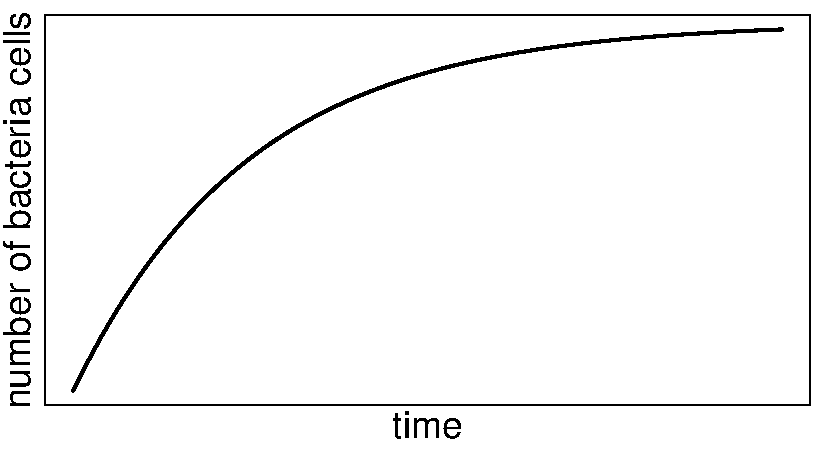
\includegraphics[width = 40mm]{ch_intro_to_data/figures/eoce/reproducing_bacteria/reproducing_bacteria_sketch.pdf}}

% 43

\eocesol{(a)~Population mean, $\mu_{2007} = 52$; sample mean, $\bar{x}_{2008} = 58$.
(b)~Population mean, $\mu_{2001} = 3.37$; sample mean, $\bar{x}_{2012} = 3.59$.}

% 45

\eocesol{Any 10 employees whose average number of days off is between the minimum and the mean
number of days off for the entire workforce at this plant.}

% 47

\eocesol{(a)~Dist~2 has a higher mean since $20 > 13$, and a higher standard deviation
since 20 is further from the rest of the data than 13.
(b)~Dist~1 has a higher mean since $-20 > -40$, and Dist~2 has a
higher standard deviation since -40 is farther away from the rest of the data than -20.
(c)~Dist~2 has a higher mean since all values in this distribution are higher
than those in Dist~1, but both distribution have the same standard deviation
since they are equally variable around their respective means.
(d)~Both distributions have the same mean since they're both centered at 300, but
Dist~2 has a higher standard deviation since the observations are farther from
the mean than in Dist~1.}

% 49

\eocesol{(a)~Q1 $\approx$ 5, median $\approx$ 15, Q3 $\approx$ 35
(b)~Since the distribution is right skewed, we would expect the mean to be higher than the median.}

% 51

\eocesol{(a)~About 30.
(b)~Since the distribution is right skewed the mean is higher than the median.
(c)~Q1: between 15 and 20, Q3: between 35 and 40, IQR: about 20.
(d)~Values that are considered to be unusually low or high lie more than 1.5$\times$IQR
away from the quartiles. Upper fence: Q3 + 1.5 $\times$ IQR =  $37.5 + 1.5 \times 20 = 67.5$;
Lower fence: Q1 - 1.5 $\times$ IQR =  $17.5 + 1.5 \times 20 =  -12.5$; The lowest AQI
recorded is not lower than 5 and the highest AQI recorded is not higher than 65, which
are both within the fences. Therefore none of the days in this sample would be considered
to have an unusually low or high AQI.}

% 53

\eocesol{The histogram shows that the distribution is bimodal, which is not apparent in the box
plot. The box plot makes it easy to identify more precise values of observations outside
of the whiskers.}

% 55

\eocesol{(a)~The distribution of number of pets per household is likely right skewed as there is a natural boundary at 0 and only a few people have many pets. Therefore the center would be best described by the median, and variability would be best described by the IQR.
(b)~The distribution of number of distance to work is likely right skewed as there is a natural boundary at 0 and only a few people live a very long distance from work. Therefore the center would be best described by the median, and variability would be best described by the IQR.
(c)~The distribution of heights of males is likely symmetric. Therefore the center would be best described by the mean, and variability would be best described by the standard deviation.}

% 57

\eocesol{No, we would expect this distribution to be right skewed. There are two reasons
for this: (1)~there is a natural boundary at 0 (it is not possible to watch less
than 0 hours of TV), (2)~the standard deviation of the distribution is very large
compared to the mean.}

% 59

\textC{\end{multicols}
\newpage
\begin{multicols}{2}}


\eocesol{The statement ``50\% of Facebook users have over 100 friends" means that the median
number of friends is 100, which is lower than the mean number of friends (190), which
suggests a right skewed distribution for the number of friends of Facebook users.}


% 61

\eocesol{(a)~The median is a much better measure of the typical amount earned by these 42
people. The mean is much higher than the income of 40 of the 42 people. This is
because the mean is an arithmetic average and gets affected by the two extreme observations. The median does not get effected as much since it is robust to
outliers.
(b)~The IQR  is a much better measure of variability in the amounts earned by nearly
all of the 42 people. The standard deviation gets affected greatly by the two high
salaries, but the IQR is robust to these extreme observations.}

% 63

\eocesol{(a)~The distribution is unimodal and symmetric with a mean of about 25 minutes
and a standard deviation of about 5 minutes. There does not appear to be any
counties with unusually high or low mean travel times. Since the distribution
is already unimodal and symmetric, a log transformation is not necessary.
(b)~Answers will vary. There are pockets of longer travel time around DC,
Southeastern NY, Chicago, Minneapolis, Los Angeles, and many other big cities.
There is also a large section of shorter average commute times that overlap
with farmland in the Midwest. Many farmers' homes are adjacent to their
farmland, so their commute would be brief, which may explain why the
average commute time for these counties is relatively low.}

% 65

\eocesol{(a)~We see the order of the categories and the relative frequencies in the bar plot.
(b)~There are no features that are apparent in the pie chart but not in the bar plot.
(c)~We usually prefer to use a bar plot as we can also see the relative frequencies of the categories in this graph.}

% 67

\eocesol{The vertical locations at which the ideological groups break into the Yes, No,
and Not Sure categories differ, which indicates that likelihood of supporting
the DREAM act varies by political ideology. This suggests that the two variables
may be dependent.}

% 69

\eocesol{(a)~(i) False. Instead of comparing counts, we should compare percentages of people in each group who suffered cardiovascular problems.
(ii)~True.
(iii)~False. Association does not imply causation. We cannot infer a causal relationship based on an observational study. The difference from part~(ii) is subtle.
(iv)~True. \\
(b)~Proportion of all patients who had cardiovascular problems: $\frac{7,979}{227,571} \approx 0.035$ \\
(c)~The expected number of heart attacks in the rosiglitazone group, if having cardiovascular problems and treatment were independent, can be calculated as the number of patients in that group multiplied by the overall cardiovascular problem rate in the study: $67,593 * \frac{7,979}{227,571} \approx 2370$. \\
(d)~(i)~$H_0$: The treatment and cardiovascular problems are independent. They have no relationship, and the difference in incidence rates between the rosiglitazone and pioglitazone groups is due to chance.
$H_A$: The treatment and cardiovascular problems are not independent. The difference in the incidence rates between the rosiglitazone and pioglitazone groups is not due to chance and rosiglitazone is associated with an increased risk of serious cardiovascular problems.
(ii)~A higher number of patients with cardiovascular problems than expected under the assumption of independence would provide support for the alternative hypothesis as this would suggest that rosiglitazone increases the risk of such problems.
(iii)~In the actual study, we observed 2,593 cardiovascular events in the rosiglitazone group. In the 1,000 simulations under the independence model, we observed somewhat less than 2,593 in every single simulation, which suggests that the actual results did not come from the independence model. That is, the variables do not appear to be independent, and we reject the independence model in favor of the alternative. The study's results provide convincing evidence that rosiglitazone is associated with an increased risk of cardiovascular problems.}



%_______________
\end{multicols}


\textC{\newpage}
